\newpage
\section{Applying $\texttt{inlabru}$ to German Cancer Data}
\label{sec:real-data}

In this second part of our analysis, we will apply the previously described approach for Bayesian analysis with the Lee-Carter (LC) and the cohort-extended Lee-Carter (LCC) model to cancer data. We will use data of German mortality of lung and stomach cancer data for the years 1999-2000. 

Firstly, we apply the LC-model to the observed lung and stomach cancer mortality rates. In this step, we compare the inference results produced by \inlabru to equivalent inference results produced by \stan. We see from the plots of the observed data in Figures \ref{fig:obs-mr-by-age} and \ref{fig:obs-mr-by-period}, that the development over time of male and female cancer mortality is quite different. Therefore, it seems reasonable to treat male and female mortality separately in our model (REFER TO MULTIVARIATE STUDY SAYING NO COMMON EFFECTS GIVE THE BEST FIT?)

% Female lung - mortality rate
\begin{figure}
    \centering
    \textbf{Female lung cancer: Estimated mortality rate - LC}
    \begin{subfigure}[b]{.85\linewidth}
        \includegraphics[width=\linewidth]{Master Thesis Code/Scripts/Real data/Output/Figures/lung_rw2_lc/female/eta_x_compared.pdf}
        \caption{The mortality rate displayed as a function of calendar year, for each age group. }
        \label{fig:eta-female_lung_lc-x}
    \end{subfigure}
    
    \begin{subfigure}[b]{.85\linewidth}
        \includegraphics[width=\linewidth]{Master Thesis Code/Scripts/Real data/Output/Figures/lung_rw2_lc/female/eta_t_compared.pdf}
        \caption{The mortality rate displayed as a function of age, for each available calendar year. }
        \label{fig:eta-female_lung_lc-t}
    \end{subfigure}
    \caption{The mortality estimated by \inlabru and \stan for female lung cancer.}
    \label{fig:eta-female_lung_lc}
\end{figure}

% Female lung - random effects
\begin{figure}
    \centering
    \textbf{Female lung cancer: Estimated random effects - LC}
    \begin{subfigure}[b]{.85\linewidth}
        \includegraphics[width=\linewidth]{Master Thesis Code/Scripts/Real data/Output/Figures/lung_rw2_lc/female/random_effects_compared.pdf}
        \caption{Estimated random effects.}
        \label{fig:random-effects-female_lung_lc-re}
    \end{subfigure}
    
    \begin{subfigure}[b]{.85\linewidth}
        \includegraphics[width=\linewidth]{Master Thesis Code/Scripts/Real data/Output/Figures/lung_rw2_lc/female/hypers_compared.pdf}
        \caption{Estimated hyperparameters}
        \label{fig:random-effects-female_lung_lc-hyper}
    \end{subfigure}
    \caption{The age and period effects as estimated by \inlabru and \stan, for female lung cancer mortality. }
    \label{fig:random-effects-female_lung_lc}
\end{figure}

% Female lung - trace plots
\begin{figure}
    \centering
    \textbf{Female lung cancer: Trace plots from \stan}
    \begin{subfigure}[b]{.45\linewidth}
        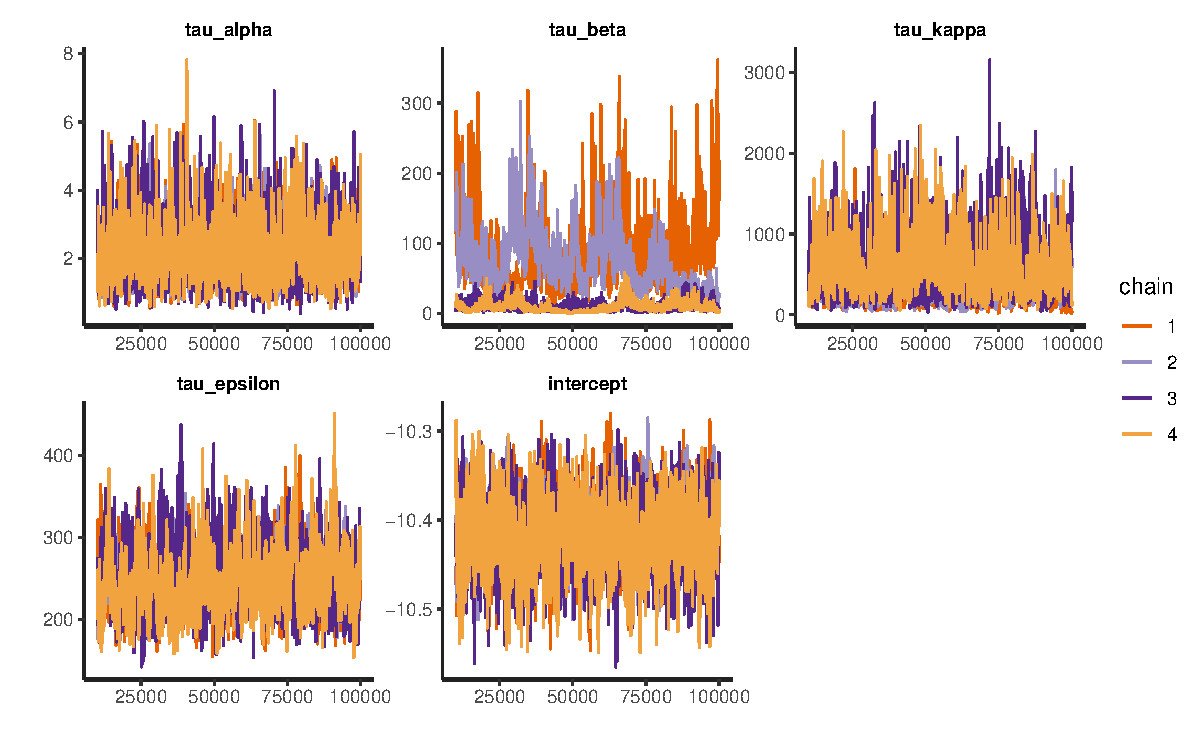
\includegraphics[width=\linewidth]{Master Thesis Code/Scripts/Real data/Stan analyses/lung_rw2_lc_female/stan_results/trace_hyperpars.pdf}
        \caption{Trace plots for hyperparameters}
        \label{fig:female-lung-lc-trace-hypers}
    \end{subfigure}
    \begin{subfigure}[b]{.45\linewidth}
        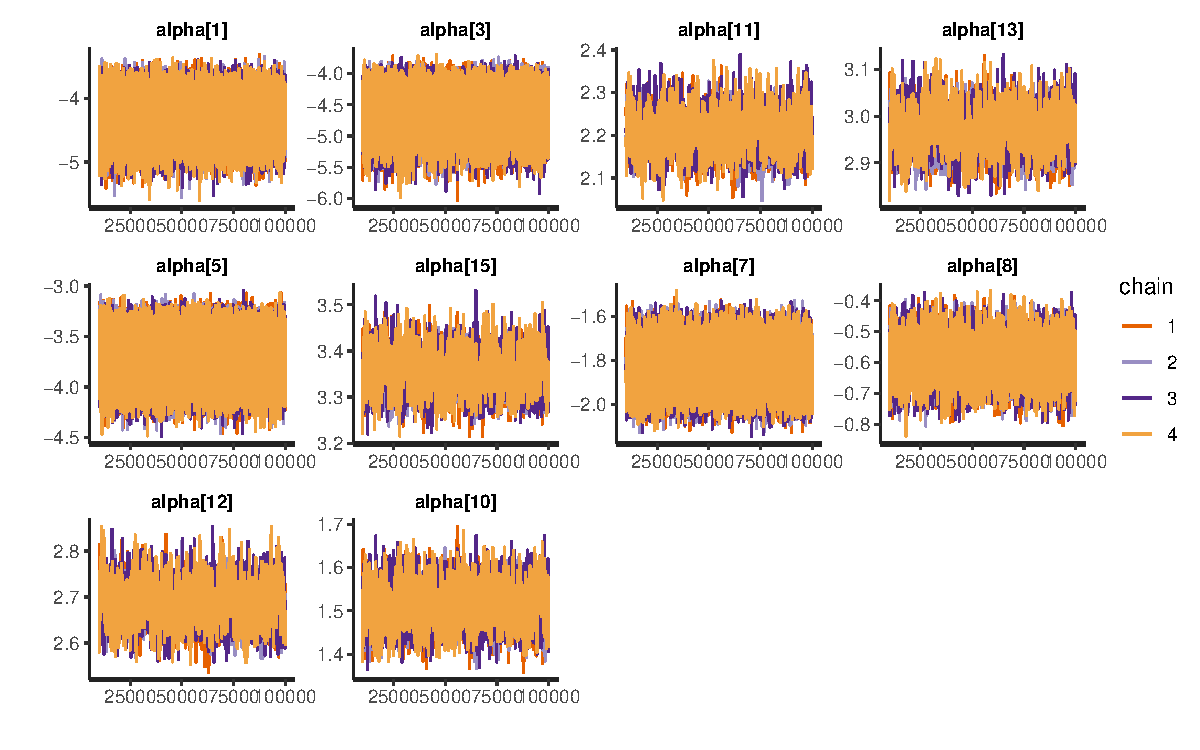
\includegraphics[width=\linewidth]{Master Thesis Code/Scripts/Real data/Stan analyses/lung_rw2_lc_female/stan_results/trace_alpha.pdf}
        \caption{Trace plots for selected values of $\alpha_x$}
        \label{fig:female-lung-lc-trace-alpha}
    \end{subfigure}
    
    \begin{subfigure}[b]{.45\linewidth}
        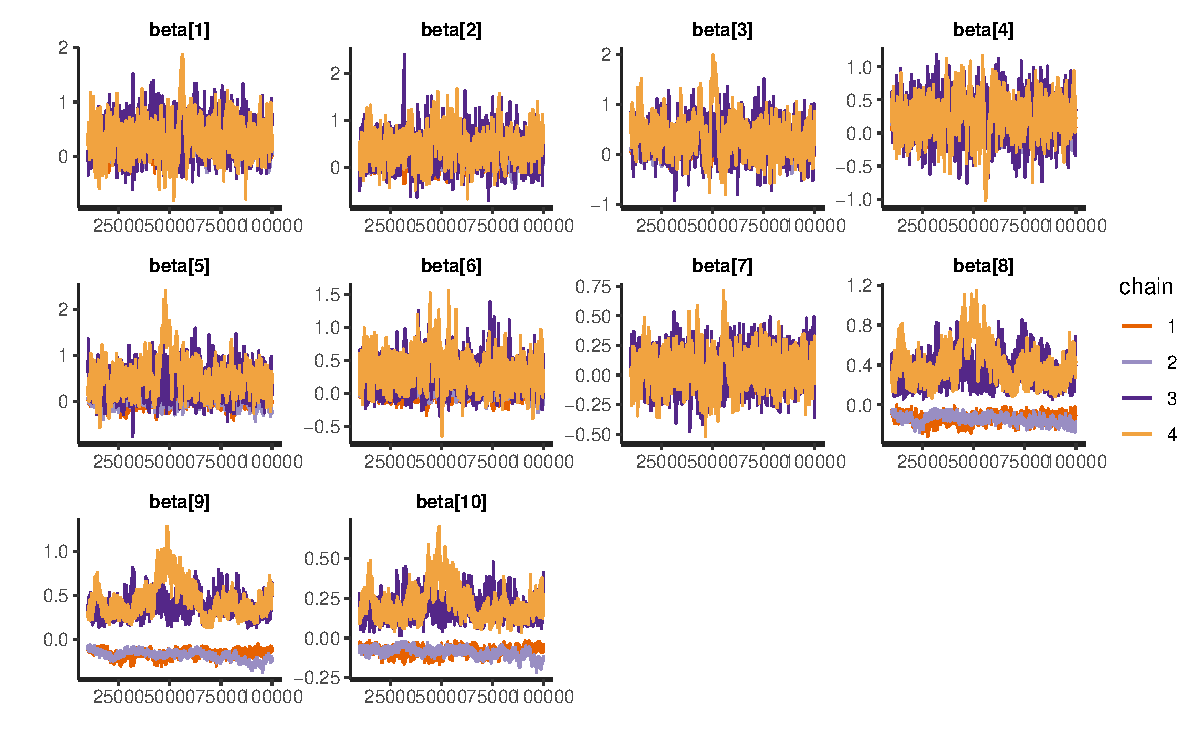
\includegraphics[width=\linewidth]{Master Thesis Code/Scripts/Real data/Stan analyses/lung_rw2_lc_female/stan_results/trace_beta.pdf}
        \caption{Trace plots for selected values of $\beta_x$}
        \label{fig:female-lung-lc-trace-beta}
    \end{subfigure}
    \begin{subfigure}[b]{.45\linewidth}
        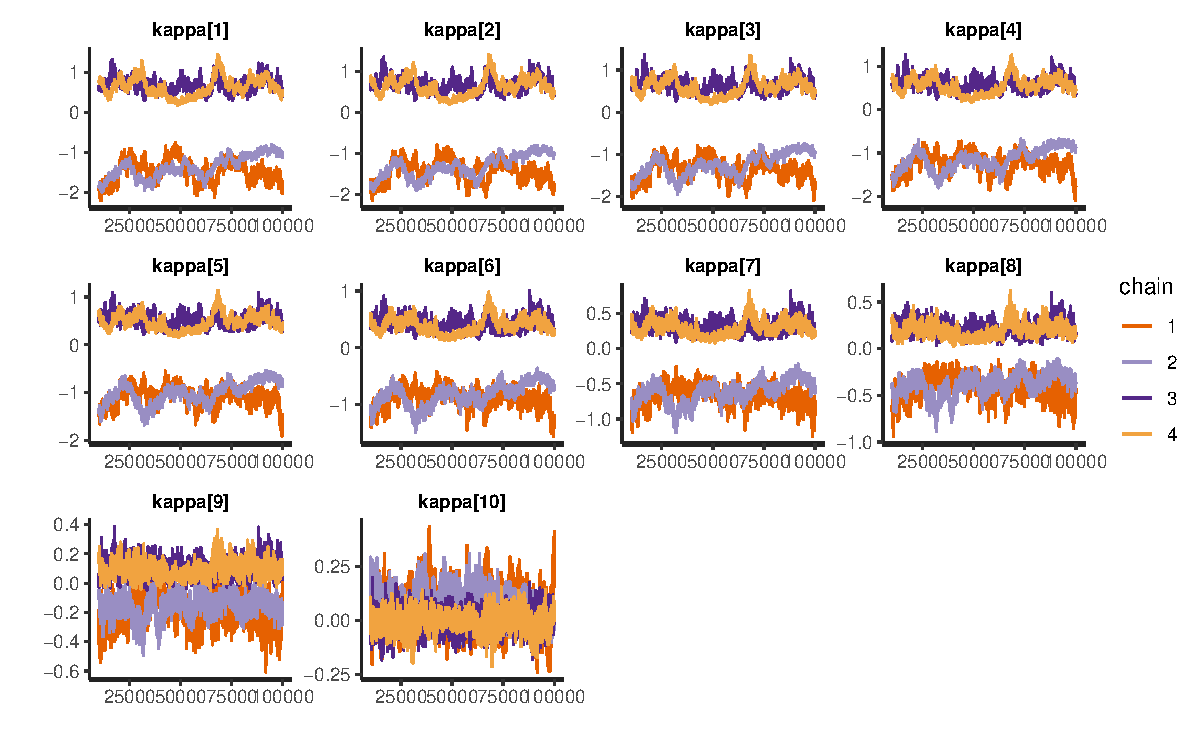
\includegraphics[width=\linewidth]{Master Thesis Code/Scripts/Real data/Stan analyses/lung_rw2_lc_female/stan_results/trace_kappa.pdf}
        \caption{Trace plots for selected values of $\kappa_t$}
        \label{fig:female-lung-lc-trace-kappa}
    \end{subfigure}
    \caption{Trace plots from inference using \stan on female lung cancer mortality. }
    \label{fig:female-lung-lc-trace}
\end{figure}

% Male lung - mortality rate
\begin{figure}
    \centering
    \textbf{Male lung cancer: Estimated mortality rate - LC}
    \begin{subfigure}[b]{.85\linewidth}
        \includegraphics[width=\linewidth]{Master Thesis Code/Scripts/Real data/Output/Figures/lung_rw2_lc/male/eta_x_compared.pdf}
        \caption{The mortality rate displayed as a function of calendar year, for each age group. }
        \label{fig:eta-male_lung_lc-x}
    \end{subfigure}
    
    \begin{subfigure}[b]{.85\linewidth}
        \includegraphics[width=\linewidth]{Master Thesis Code/Scripts/Real data/Output/Figures/lung_rw2_lc/male/eta_t_compared.pdf}
        \caption{The mortality rate displayed as a function of age, for each available calendar year. }
        \label{fig:eta-female_lung_lc-t}
    \end{subfigure}
    \caption{The mortality estimated by \inlabru and \stan for male lung cancer.}
    \label{fig:eta-male_lung_lc}
\end{figure}

% Male lung - random effects 
\begin{figure}
    \centering
    \textbf{Male lung cancer: Estimated random effects - LC}
    \begin{subfigure}[b]{.85\linewidth}
        \includegraphics[width=\linewidth]{Master Thesis Code/Scripts/Real data/Output/Figures/lung_rw2_lc/male/random_effects_compared.pdf}
        \caption{Estimated random effects.}
        \label{fig:random-effects-male_lung_lc-re}
    \end{subfigure}
    
    \begin{subfigure}[b]{.85\linewidth}
        \includegraphics[width=\linewidth]{Master Thesis Code/Scripts/Real data/Output/Figures/lung_rw2_lc/male/hypers_compared.pdf}
        \caption{Estimated hyperparameters}
        \label{fig:random-effects-male_lung_lc-hyper}
    \end{subfigure}
    \caption{The age and period effects as estimated by \inlabru and \stan, for male lung cancer mortality. }
    \label{fig:random-effects-male_lung_lc}
\end{figure}

% Male lung - trace plots
% Unavailable, weirdly saved. 

% Female stomach - mortality rate
\begin{figure}
    \centering
    \textbf{Female stomach cancer: Estimated mortality rate - LC}
    \begin{subfigure}[b]{.85\linewidth}
        \includegraphics[width=\linewidth]{Master Thesis Code/Scripts/Real data/Output/Figures/stomach_rw2_lc/female/eta_x_compared.pdf}
        \caption{The mortality rate displayed as a function of calendar year, for each age group. }
        \label{fig:eta-female_stomach_lc-x}
    \end{subfigure}
    
    \begin{subfigure}[b]{.85\linewidth}
        \includegraphics[width=\linewidth]{Master Thesis Code/Scripts/Real data/Output/Figures/stomach_rw2_lc/female/eta_t_compared.pdf}
        \caption{The mortality rate displayed as a function of age, for each available calendar year. }
        \label{fig:eta-female_stomach_lc-t}
    \end{subfigure}
    \caption{The mortality estimated by \inlabru and \stan for female stomach cancer.}
    \label{fig:eta-female_stomach_lc}
\end{figure}

% Female stomach - random effects
\begin{figure}
    \centering
    \textbf{Female stomach cancer: Estimated random effects - LC}
    \begin{subfigure}[b]{.85\linewidth}
        \includegraphics[width=\linewidth]{Master Thesis Code/Scripts/Real data/Output/Figures/stomach_rw2_lc/female/random_effects_compared.pdf}
        \caption{Estimated random effects.}
        \label{fig:random-effects-female_stomach_lc-re}
    \end{subfigure}
    
    \begin{subfigure}[b]{.85\linewidth}
        \includegraphics[width=\linewidth]{Master Thesis Code/Scripts/Real data/Output/Figures/stomach_rw2_lc/female/hypers_compared.pdf}
        \caption{Estimated hyperparameters}
        \label{fig:random-effects-female_stomach_lc-hyper}
    \end{subfigure}
    \caption{The age and period effects as estimated by \inlabru and \stan for female stomach cancer mortality. }
    \label{fig:random-effects-female_stomach_lc}
\end{figure}

% Female stomach - trace plots
\begin{figure}
    \centering
    \textbf{Female stomach cancer: Trace plots from \stan}
    \begin{subfigure}[b]{.45\linewidth}
        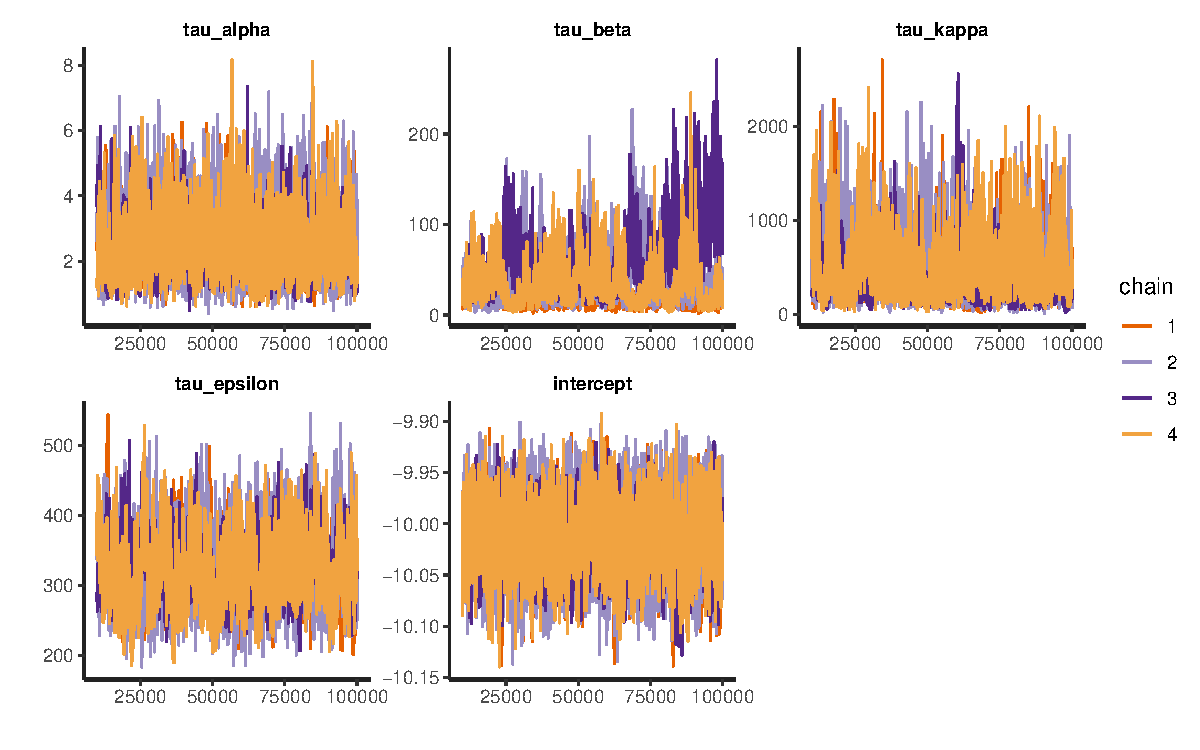
\includegraphics[width=\linewidth]{Master Thesis Code/Scripts/Real data/Stan analyses/stomach_rw2_lc_female/stan_results/trace_hyperpars.pdf}
        \caption{Trace plots for hyperparameters}
        \label{fig:female-stomach-lc-trace-hypers}
    \end{subfigure}
    \begin{subfigure}[b]{.45\linewidth}
        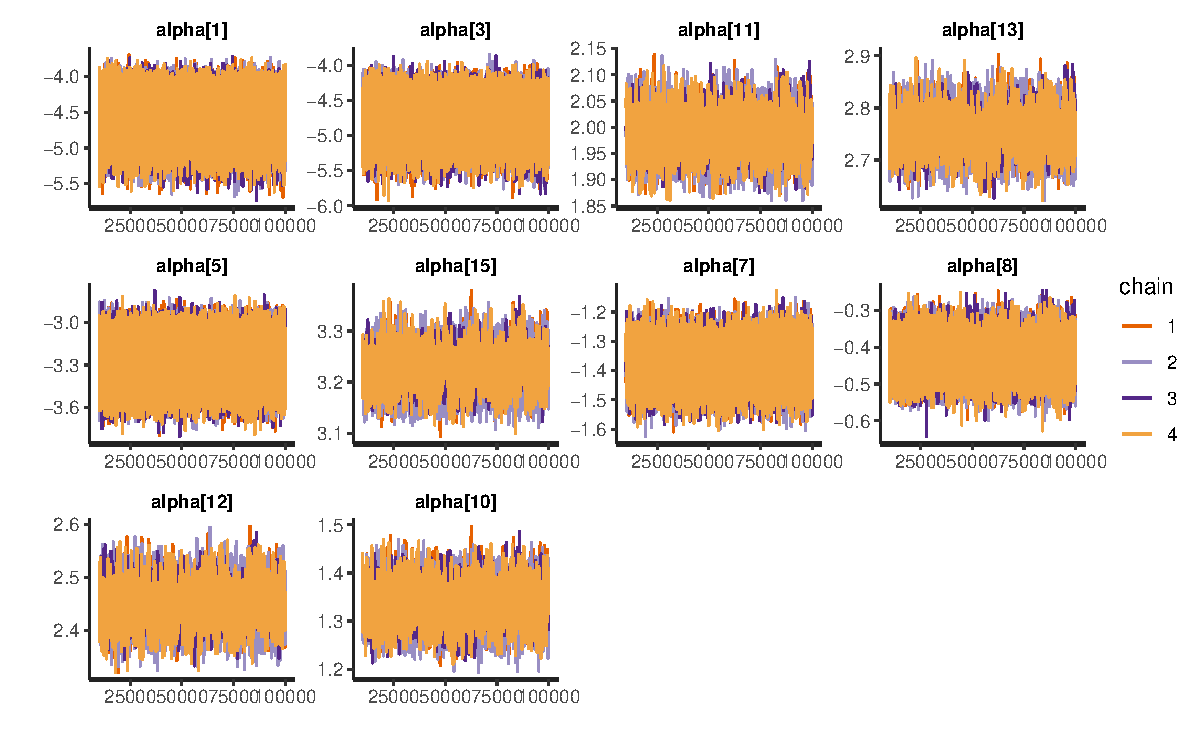
\includegraphics[width=\linewidth]{Master Thesis Code/Scripts/Real data/Stan analyses/stomach_rw2_lc_female/stan_results/trace_alpha.pdf}
        \caption{Trace plots for selected values of $\alpha_x$}
        \label{fig:female-stomach-lc-trace-alpha}
    \end{subfigure}
    
    \begin{subfigure}[b]{.45\linewidth}
        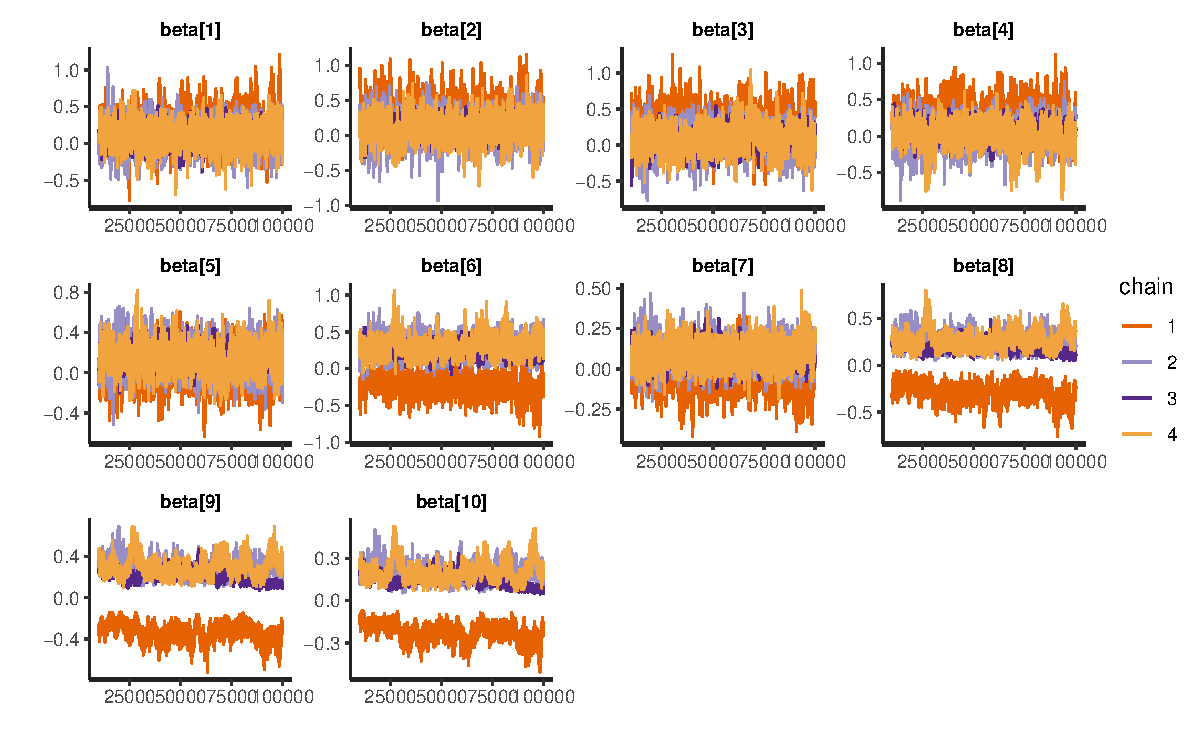
\includegraphics[width=\linewidth]{Master Thesis Code/Scripts/Real data/Stan analyses/stomach_rw2_lc_female/stan_results/trace_beta.pdf}
        \caption{Trace plots for selected values of $\beta_x$}
        \label{fig:female-stomach-lc-trace-beta}
    \end{subfigure}
    \begin{subfigure}[b]{.45\linewidth}
        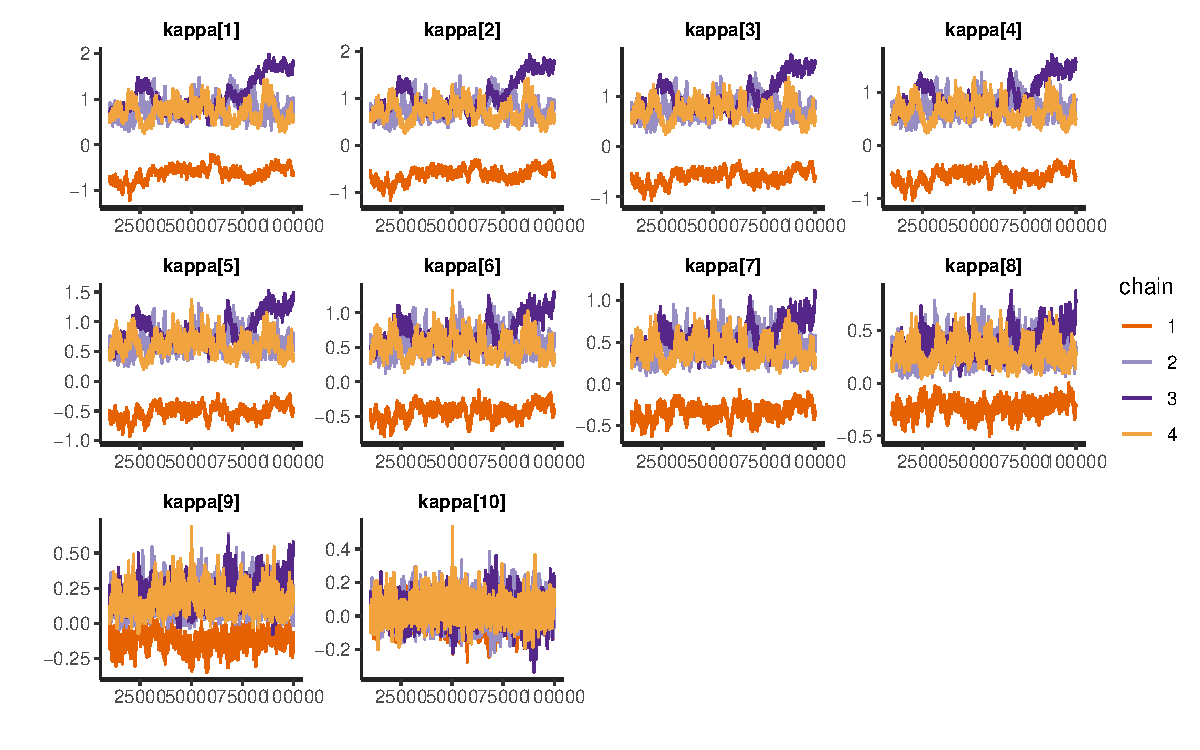
\includegraphics[width=\linewidth]{Master Thesis Code/Scripts/Real data/Stan analyses/stomach_rw2_lc_female/stan_results/trace_kappa.pdf}
        \caption{Trace plots for selected values of $\kappa_t$}
        \label{fig:female-stomach-lc-trace-kappa}
    \end{subfigure}
    \caption{Trace plots from inference using \stan on female stomach cancer mortality. }
    \label{fig:female-stomach-lc-trace}
\end{figure}

% Male stomach - mortality rate
\begin{figure}
    \centering
    \textbf{Male stomach cancer: Estimated mortality rate - LC}
    \begin{subfigure}[b]{.85\linewidth}
        \includegraphics[width=\linewidth]{Master Thesis Code/Scripts/Real data/Output/Figures/stomach_rw2_lc/male/eta_x_compared.pdf}
        \caption{The mortality rate displayed as a function of calendar year, for each age group. }
        \label{fig:eta-male_stomach_lc-x}
    \end{subfigure}
    
    \begin{subfigure}[b]{.85\linewidth}
        \includegraphics[width=\linewidth]{Master Thesis Code/Scripts/Real data/Output/Figures/stomach_rw2_lc/male/eta_t_compared.pdf}
        \caption{The mortality rate displayed as a function of age, for each available calendar year. }
        \label{fig:eta-male_stomach_lc-t}
    \end{subfigure}
    \caption{The mortality estimated by \inlabru and \stan for male stomach cancer.}
    \label{fig:eta-male_stomach_lc}
\end{figure}

% Male stomach - random effects
\begin{figure}
    \centering
    \textbf{Male stomach cancer: Estimated random effects - LC}
    \begin{subfigure}[b]{.85\linewidth}
        \includegraphics[width=\linewidth]{Master Thesis Code/Scripts/Real data/Output/Figures/stomach_rw2_lc/male/random_effects_compared.pdf}
        \caption{Estimated random effects.}
        \label{fig:random-effects-male_stomach_lc-re}
    \end{subfigure}
    
    \begin{subfigure}[b]{.85\linewidth}
        \includegraphics[width=\linewidth]{Master Thesis Code/Scripts/Real data/Output/Figures/stomach_rw2_lc/male/hypers_compared.pdf}
        \caption{Estimated hyperparameters}
        \label{fig:random-effects-male_stomach_lc-hyper}
    \end{subfigure}
    \caption{The age and period effects as estimated by \inlabru and \stan for male stomach cancer mortality. }
    \label{fig:random-effects-male_stomach_lc}
\end{figure}

% Male stomach - trace plots
\begin{figure}
    \centering
    \textbf{Male stomach cancer: Trace plots from \stan}
    \begin{subfigure}[b]{.45\linewidth}
        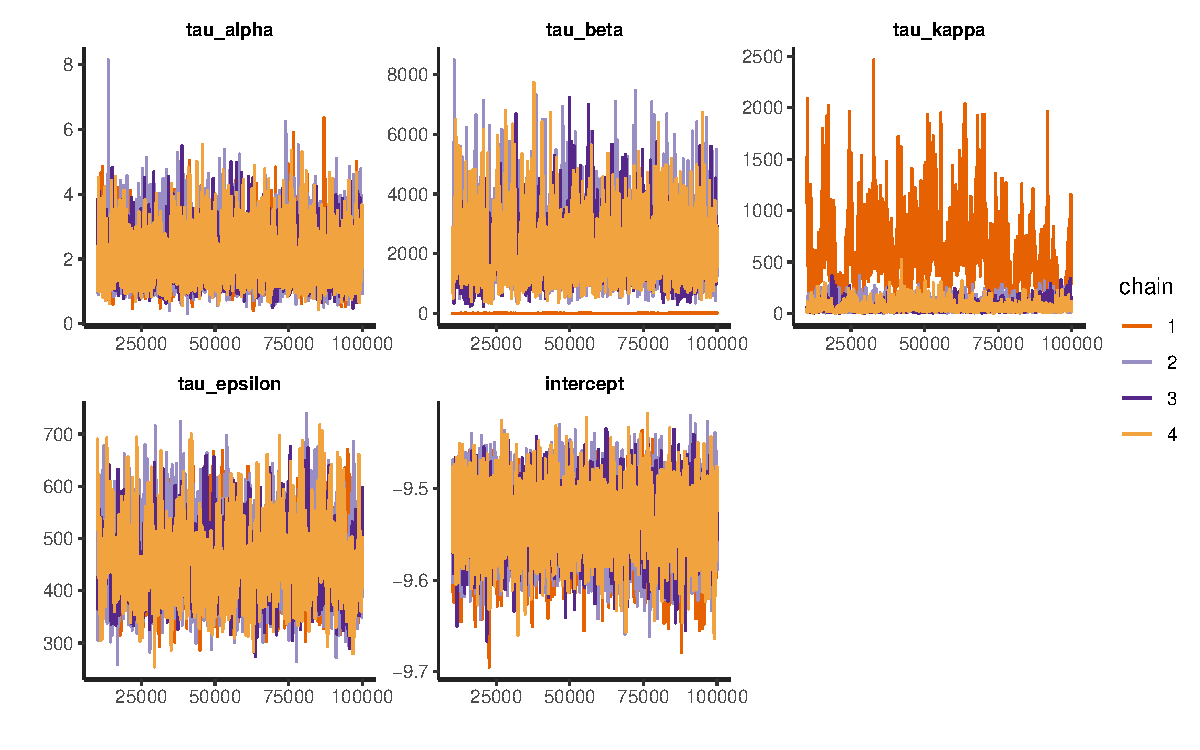
\includegraphics[width=\linewidth]{Master Thesis Code/Scripts/Real data/Stan analyses/stomach_rw2_lc_male/stan_results/trace_hyperpars.pdf}
        \caption{Trace plots for hyperparameters}
        \label{fig:male-stomach-lc-trace-hypers}
    \end{subfigure}
    \begin{subfigure}[b]{.45\linewidth}
        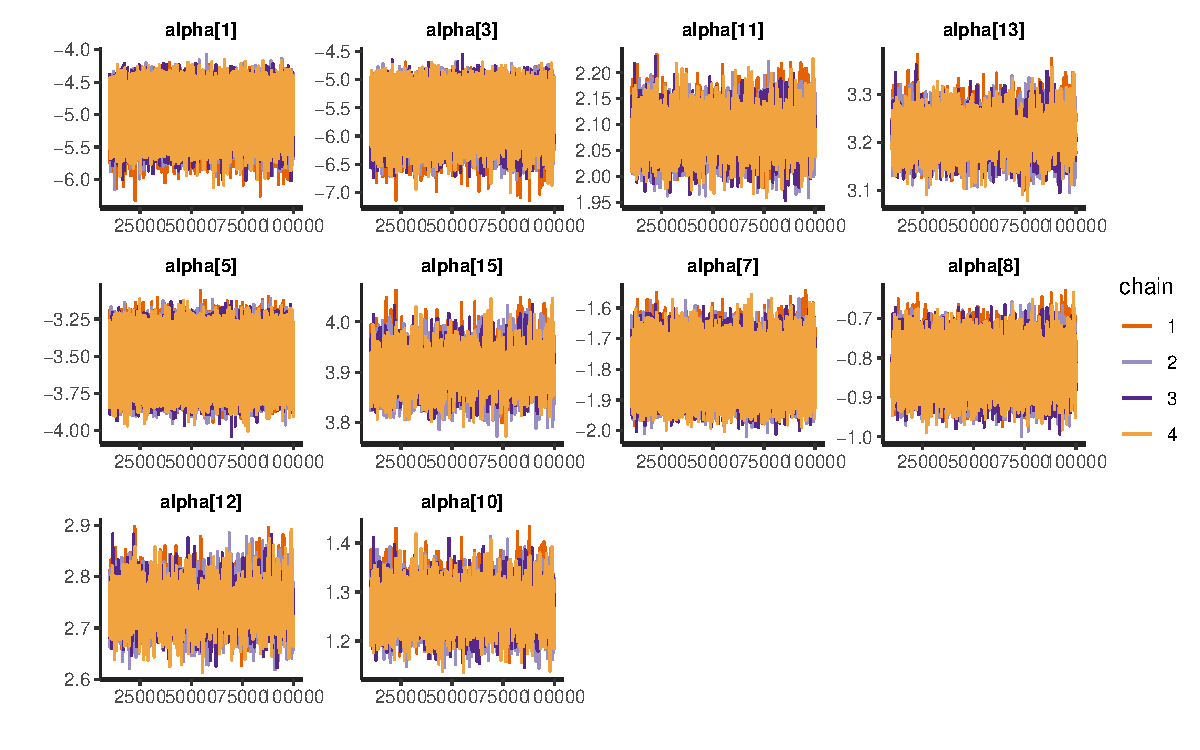
\includegraphics[width=\linewidth]{Master Thesis Code/Scripts/Real data/Stan analyses/stomach_rw2_lc_male/stan_results/trace_alpha.pdf}
        \caption{Trace plots for selected values of $\alpha_x$}
        \label{fig:male-stomach-lc-trace-alpha}
    \end{subfigure}
    
    \begin{subfigure}[b]{.45\linewidth}
        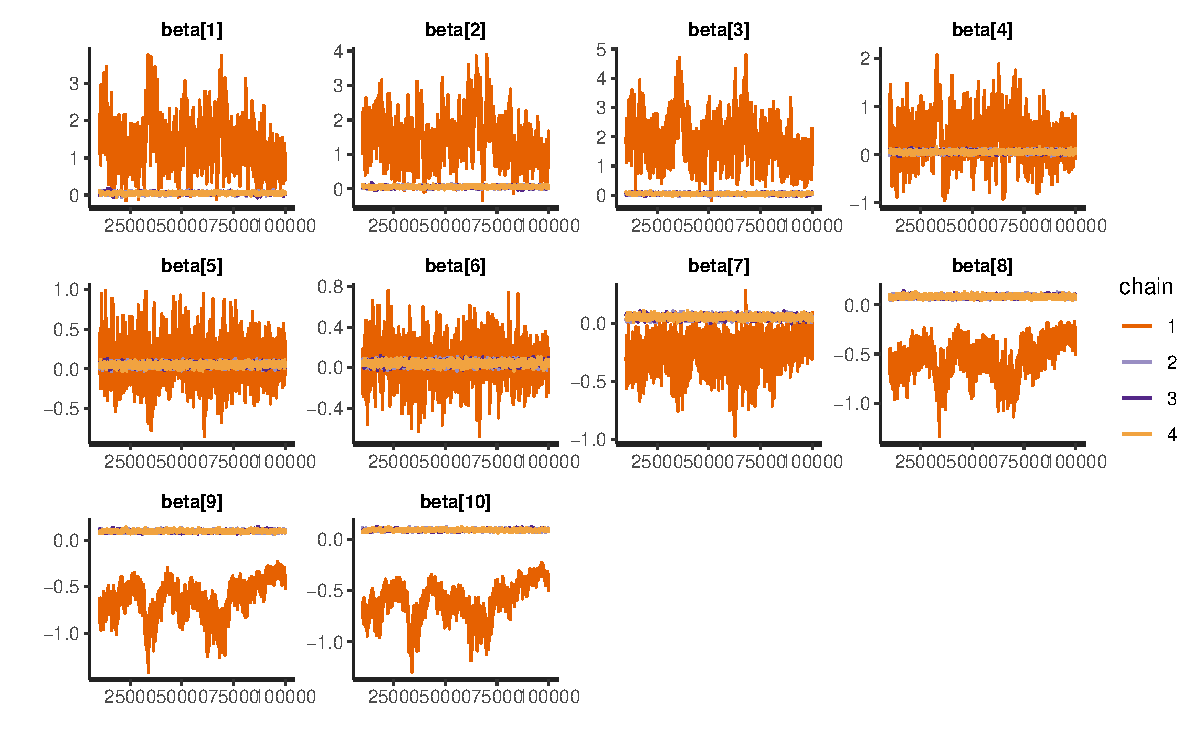
\includegraphics[width=\linewidth]{Master Thesis Code/Scripts/Real data/Stan analyses/stomach_rw2_lc_male/stan_results/trace_beta.pdf}
        \caption{Trace plots for selected values of $\beta_x$}
        \label{fig:male-stomach-lc-trace-beta}
    \end{subfigure}
    \begin{subfigure}[b]{.45\linewidth}
        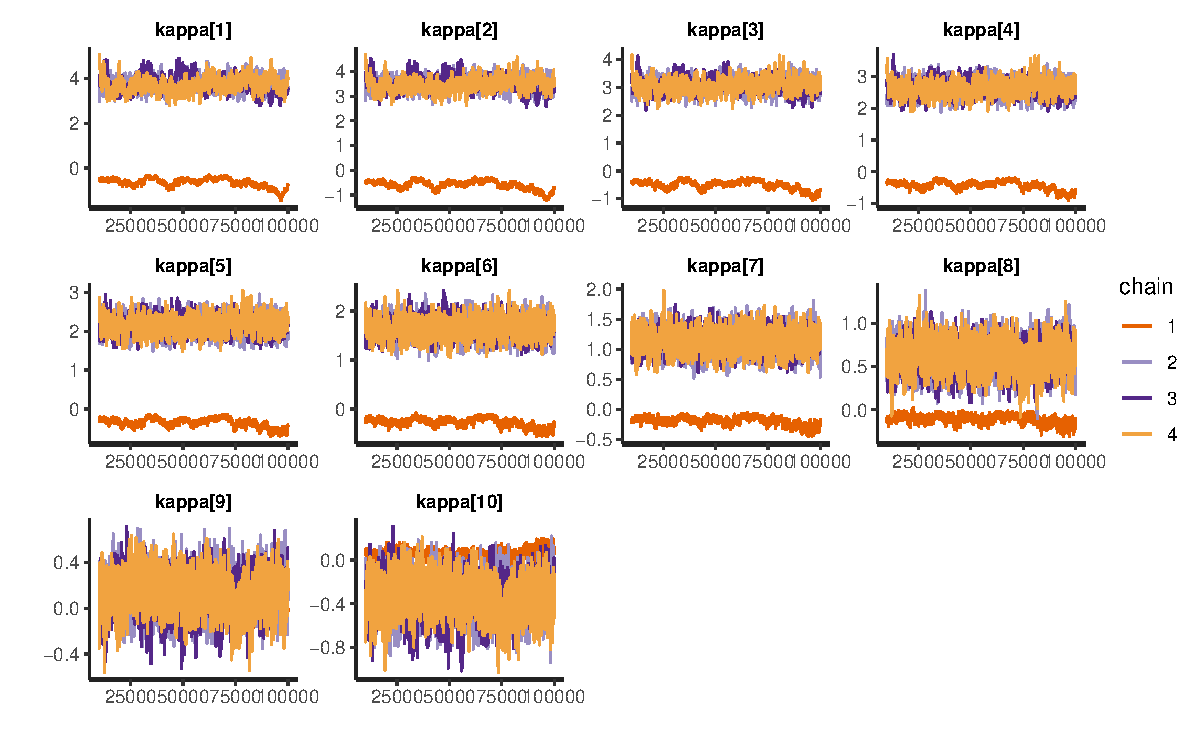
\includegraphics[width=\linewidth]{Master Thesis Code/Scripts/Real data/Stan analyses/stomach_rw2_lc_male/stan_results/trace_kappa.pdf}
        \caption{Trace plots for selected values of $\kappa_t$}
        \label{fig:male-stomach-lc-trace-kappa}
    \end{subfigure}
    \caption{Trace plots from inference using \stan on male stomach cancer mortality. }
    \label{fig:male-stomach-lc-trace}
\end{figure}



Figures \ref{fig:mr-lcc-stomach} and \ref{fig:random-effects-lcc-stomach} displays the stomach cancer mortality rates and age, period and cohort effects, with their associated hyperparameters, as estimated by $\texttt{inlabru}$ for the LCC-model. These results are produced in the script \url{Master Thesis Code/Scripts/Real data/run_inlabru_real_data.R}.

\begin{figure}
    \centering
    \textbf{LCC-model: estimated mortality rates for stomach cancer}
    \begin{subfigure}[b]{.45\linewidth}
        \includegraphics[width=\linewidth]{Master Thesis Code/Scripts/Real data/Output/Figures/stomach_rw2/mr_x_inlabru.pdf}
        \caption{Mortality rates displayed as a function of calendar year, for each age group. }
        \label{fig:mr-lcc-stomach-x}
    \end{subfigure}
    \begin{subfigure}[b]{.45\linewidth}
        \includegraphics[width=\linewidth]{Master Thesis Code/Scripts/Real data/Output/Figures/stomach_rw2/mr_t_inlabru.pdf}
        \caption{The mortality rates displayed as a function of age, for each available calendar year. }
        \label{fig:mr-lcc-stomach-t}
    \end{subfigure}
    \caption{The stomach cancer mortality rate estimated by $\texttt{inlabru}$ displayed together with the observed stomach cancer mortality rate.}
    \label{fig:mr-lcc-stomach}
\end{figure}

\begin{figure}
    \centering
    \textbf{LCC-model: estimated age, period and cohort effects for stomach cancer}
    \begin{subfigure}[b]{.85\linewidth}
        \includegraphics[width=\linewidth]{Master Thesis Code/Scripts/Real data/Output/Figures/stomach_rw2/random_effects_inlabru.pdf}
        \caption{Estimated random effects.}
        \label{fig:random-effects-lcc-stomach-re}
    \end{subfigure}
    
    \begin{subfigure}[b]{.85\linewidth}
        \includegraphics[width=\linewidth]{Master Thesis Code/Scripts/Real data/Output/Figures/stomach_rw2/hypers_inlabru.pdf}
        \caption{Estimated hyperparameters}
        \label{fig:random-effects-lcc-stomach-hyper}
    \end{subfigure}
    \caption{The random age- period and cohort effects, as well as the hyperparameters, estimated by applying the LCC-model to stomach cancer mortality data by $\texttt{inlabru}$.}
    \label{fig:random-effects-lcc-stomach}
\end{figure}

Figures \ref{fig:mr-lcc-lung} and \ref{fig:random-effects-lcc-lung} displays the lung cancer mortality rates and age, period and cohort effects, with their associated hyperparameters, as estimated by $\texttt{inlabru}$ for the LDD-model. These results are produced in the script \url{Master Thesis Code/Scripts/Real data/run_inlabru_real_data.R}.

\begin{figure}
    \centering
    \textbf{LCC-model: estimated mortality rates for lung cancer}
    \begin{subfigure}[b]{.45\linewidth}
        \includegraphics[width=\linewidth]{Master Thesis Code/Scripts/Real data/Output/Figures/lung_rw2/mr_x_inlabru.pdf}
        \caption{Mortality rates displayed as a function of calendar year, for each age group. }
        \label{fig:mr-lcc-lung-x}
    \end{subfigure}
    \begin{subfigure}[b]{.45\linewidth}
        \includegraphics[width=\linewidth]{Master Thesis Code/Scripts/Real data/Output/Figures/lung_rw2/mr_t_inlabru.pdf}
        \caption{The mortality rates displayed as a function of age, for each available calendar year. }
        \label{fig:mr-lcc-lung-t}
    \end{subfigure}
    \caption{The lung cancer mortality rate estimated by $\texttt{inlabru}$ displayed together with the observed lung cancer mortality rate.}
    \label{fig:mr-lcc-lung}
\end{figure}

\begin{figure}
    \centering
    \textbf{LCC-model: estimated age, period and cohort effects for lung cancer}
    \begin{subfigure}[b]{.85\linewidth}
        \includegraphics[width=\linewidth]{Master Thesis Code/Scripts/Real data/Output/Figures/lung_rw2/random_effects_inlabru.pdf}
        \caption{Estimated random effects.}
        \label{fig:random-effects-lcc-lung-re}
    \end{subfigure}
    
    \begin{subfigure}[b]{.85\linewidth}
        \includegraphics[width=\linewidth]{Master Thesis Code/Scripts/Real data/Output/Figures/lung_rw2/hypers_inlabru.pdf}
        \caption{Estimated hyperparameters}
        \label{fig:random-effects-lcc-lung-hyper}
    \end{subfigure}
    \caption{The age- period and cohort effects, as well as the hyperparameters, estimated by applying the LCC-model to lung cancer mortality data by $\texttt{inlabru}$.}
    \label{fig:random-effects-lcc-lung}
\end{figure}